\documentclass{../template/tp}
\usepackage[utf8x]{inputenc}

\usepackage[frenchb]{babel}
\usepackage[T1]{fontenc}

\usepackage{graphicx}
\usepackage{amssymb}
\usepackage{amsmath}
\usepackage{wasysym} %smiley
\usepackage{hyperref}% hyperliens
\usepackage{tikz}
\usetikzlibrary{babel,positioning,calc}
\usepackage[]{circuitikz}
\usepackage{textcomp}
% \usepackage{minted}
\usepackage[long]{datetime}
\usepackage{gensymb} % \ohm, celsius
\usepackage{framed}
\usepackage{pdfpages}
\usepackage{todo}
\usepackage{fancyhdr}

% \langexam{frenchb}

\newboolean{koriG}
\ifx\koriG\undefined
\correction{false}
\else
\correction{true}
\fi

% \correction{false}
%  \correction{true}

%% fancy header & foot
\pagestyle{fancy}
\lhead{[ELEC-H-301] Électronique appliquée\\ TP \no 6 : analyse de problèmes d’électronique\ifthenelse{\boolean{corrige}}{~-- Corrigé}{}}
\rhead{v1.1.2\\ page \thepage}
\cfoot{}
%%

\pdfinfo{
/Author (ULB -- BEAMS)
/Title (TP 6 ELEC-H-301, analyse de problèmes d’électronique)
/ModDate (D:\pdfdate)

}
\hypersetup{
pdftitle={TP 6 [ELEC-H-301] Électronique appliquée : analyse de problèmes d’électronique},
pdfauthor={ULB - BEAMS  },
pdfsubject={analyse de problèmes d’électronique}
}

\author{The Fantastic Four}

\begin{document}

\tptitle{ELEC-H-301~: Électronique appliquée}{Séance 6~: analyse de problèmes d’électronique}

% \todo{Arranger l'ordre des exercices}

Cette séance d'exercices a pour objectifs de vous apprendre à:
\begin{itemize}
\item Bien contextualiser les problèmes d'électronique vus cette année.
\item Sélectionner les bonnes méthodes de résolution de circuits électroniques.
\end{itemize}



% Q1.1
%\Question{
%Calculate the reactance of a $1\mu F$ capacitor at a frequency of $10kHz$, and the reactance of a $20mH$ inductor at a frequency of $100rad/s$. In each case include the units in your answer.
%}%
%{
%}

\section*{Le chronomètre du projet BA2}
Le but de ce problème est de concevoir une barrière photoélectrique pour détecter (et chronométrer) les robots du projet BA2 de la filière Electromec pour l'année 2016-2017.

Le dispositif est constitué comme suit :

%emetteur
%led
%miroir
%recepteur
%sortie\marginpar{faire schéma émetteur + led + IR + pd + recepteur + info de sortie}
\begin{center}
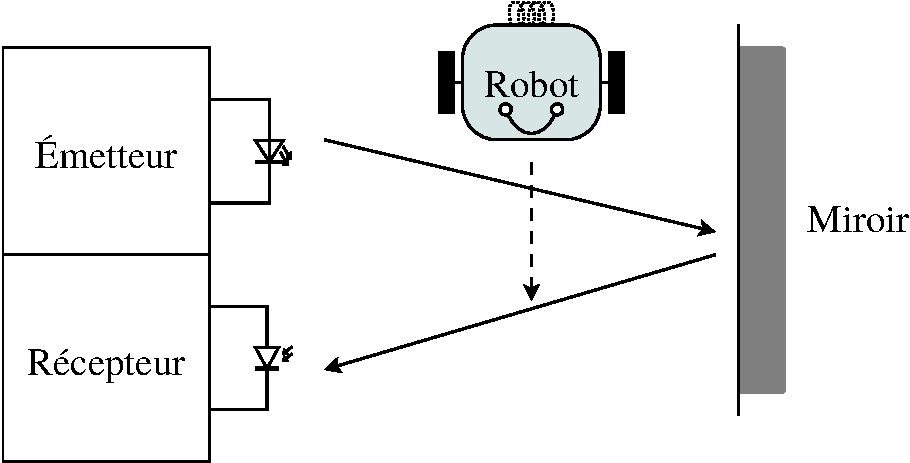
\includegraphics[width=8cm]{ER_ir-crop.pdf}
\end{center}

Pour améliorer la fiabilité de la barrière photoélectrique, le faisceau infra-rouge sera modulé.

Toutes les questions du problème sont \textbf{indépendantes}, il n'est pas nécessaire d'avoir répondu aux questions précédentes pour répondre à une question. 

L'émetteur et le récepteur seront étudiés séparément, respectivement aux sections \ref{Q:emetteur} et \ref{Q:recepteur}. Pour le récepteur, les différentes questions portent sur différents étages et sont indépendantes du contexte du problème.
\newpage



\section{Chronomètre: émetteur}
L'émetteur est constitué d'une source de tension $E1$ produisant un signal rectangulaire 0--5V à 10kHz, rapport cyclique 10\% :
\label{Q:emetteur}
\begin{center}
%\shorthandoff{:!}
		\begin{circuitikz}%\draw
			\draw		
			(0,0) to [square voltage source, l=$E1$] (0,2) to [R, l=$R$] (2,2) to [led, l_=$D$](2,0) --(0,0)
			;
		\end{circuitikz}
		%\shorthandon{:!}
	\end{center}
    
%\newpage


{\color{white} Cet énoncé est un prototype de question d'examen, have fun! }
\Question
{
%question
Sur base de la documentation fournie page suivante, dimensionnez $R$ de façon à limiter le courant dans la diode à 100mA.
}
{%answer
La courbe $I_F=f(V_F)$ permet de constater que $V_F=1.35V$ pour $I_F=100mA$, par conséquent $R=\frac{E-V_F}{I_F}=36.5\Omega$.
}
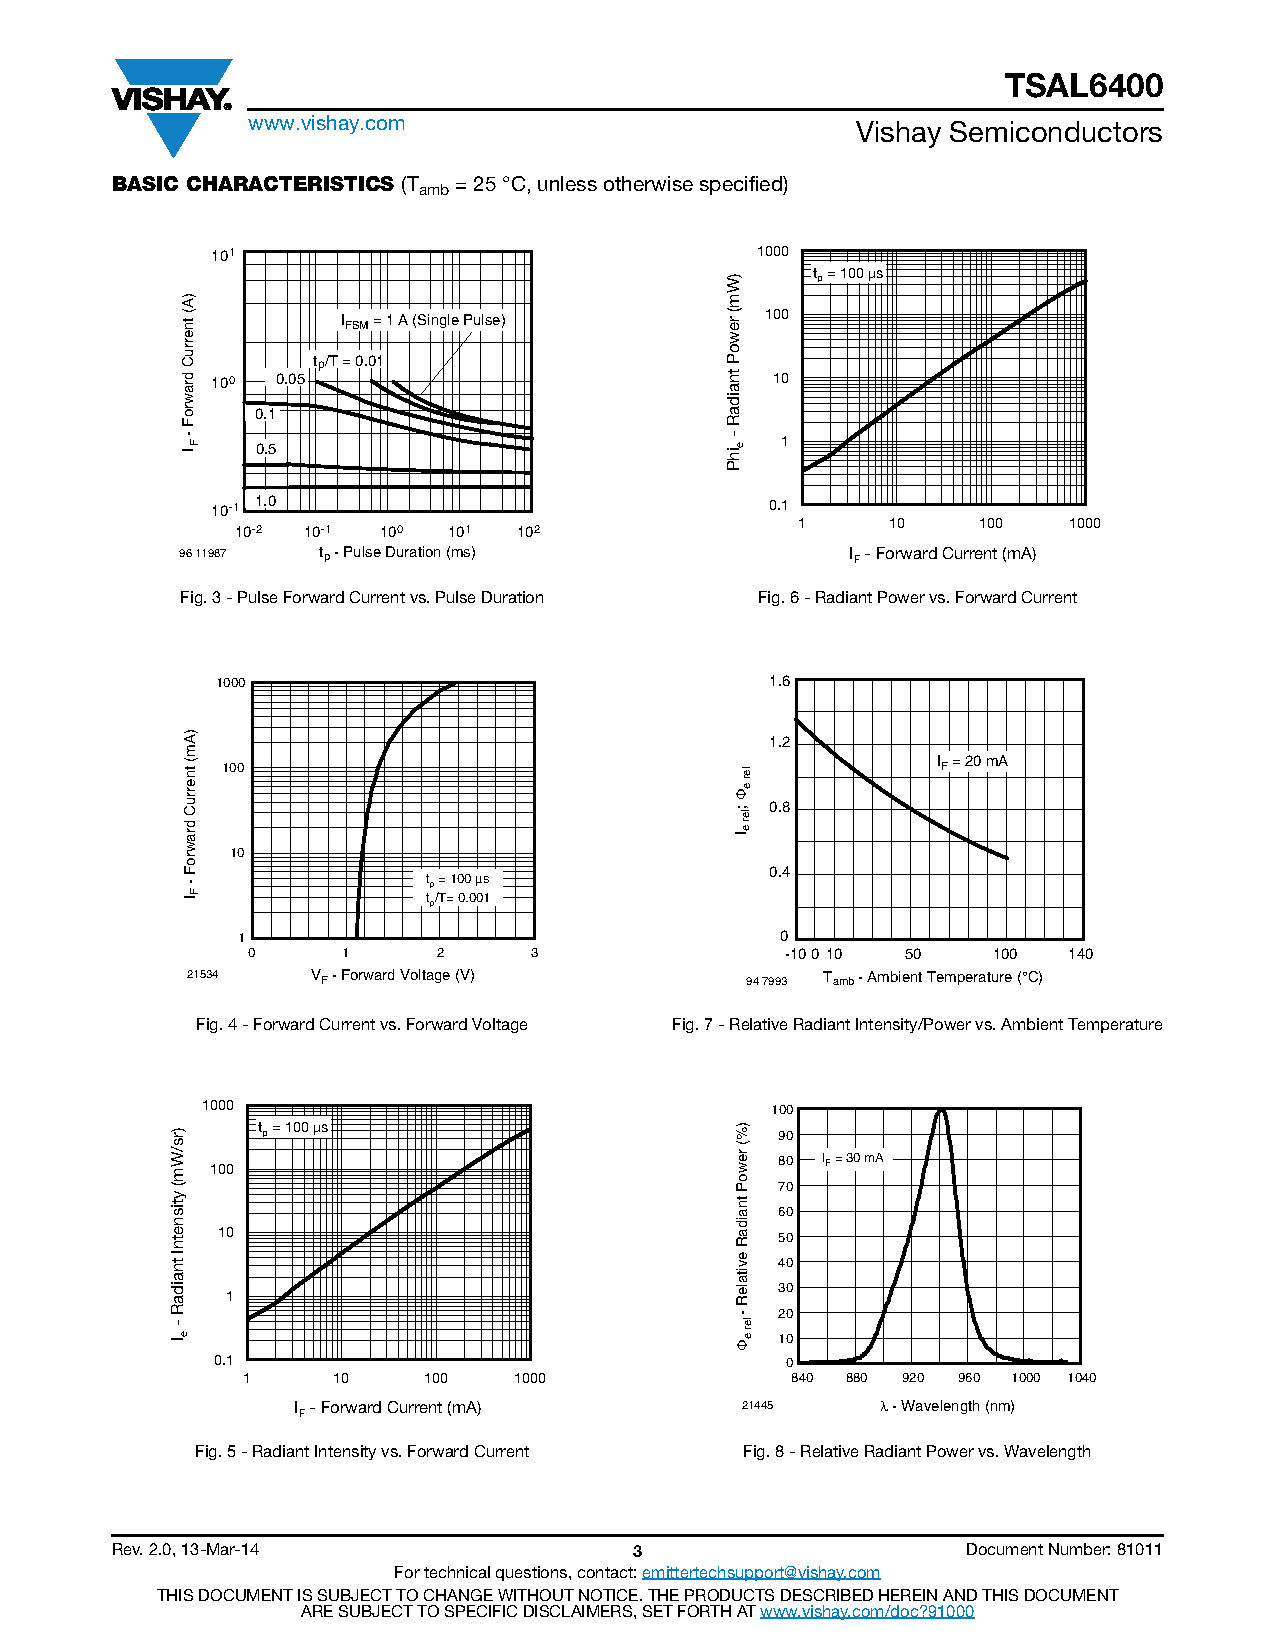
\includepdf[pages={1},scale=0.9,pagecommand={\pagestyle{plain}}]{doc_led.pdf}



\section{Chronomètre: récepteur}
 Le capteur infrarouge utilisé est une photodiode et nous allons l'utiliser comme source de tension.
\label{Q:recepteur}
Le récepteur est constitué de multiples blocs (voir schéma ci-dessous):
 \begin{itemize}
 \item photodiode (=capteur infra-rouge)
 \item amplificateur
 \item filtre
 \item deuxième amplificateur %(non étudié dans cet examen)
 \item comparateur
 \item circuits logiques de sortie, deux sorties logiques :
 \begin{itemize}
 \item "Pas d'obstacle" indique que le faisceau est établi entre l'émetteur et le récepteur.
 \item "Éblouissement" indique que le circuit n'est plus capable de décider si le faisceau est établi parce que l'éclairage ambiant est trop important et/ou un signal parasite perturbe la mesure (malgré la modulation). %Cette sortie ne sera pas étudiée dans cet examen.
 \end{itemize}
 \end{itemize}

\begin{center}
 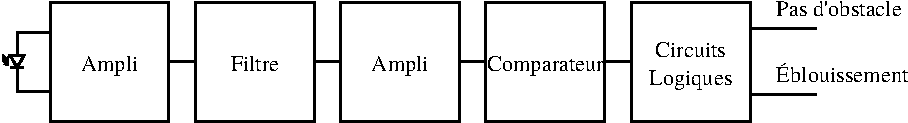
\includegraphics[width=12cm]{recepteur-crop.pdf}
 \end{center}


\subsection{Photodiode+amplificateur}
Les deux premiers étages du récepteur forment le circuit ci-dessous.

La photodiode est assimilable à une source de tension dont l'amplitude est proportionnelle à la puissance lumineuse reçue et vaut environ 0.5V en moyenne dans une pièce correctement éclairée.

\begin{center}
\shorthandoff{:!}
\begin{circuitikz}%\draw
			\draw	
%			(0,6) to [short,i=$I$] 
			(0,4.5) to [photodiode,v_<=$V_D$, ] (0,0) node [ground] {}
%			  (-2,0) node [ground] {}to [european voltage source,v=$ $,l_=$\equiv V_{D}$ ](-2,4.5) to [short] (-1,4.5) 
			(4,4) node[op amp, yscale=-1] (opamp) {}
            % (opamp.+) node[left] {$v_+$}
            % (opamp.-) node[left] {$v_-$}
            % (opamp.out) node[right] {$v_o$}
			(opamp.down) ++ (0,+0.5) node[above] {12V} -- (opamp.down)
			 (opamp.up) ++ (0,-0.5) node[below] {-12V} -- (opamp.up)
			 (opamp.-) -| ++(-0.5,-1.5) to [R, l_=$R_2$] ++(2.75,0) -|  (opamp.out)
			 (opamp.-) -| ++(-0.5,-1.5) to [R, l=$R_1$] (2.25,0) node[ground] {}
			 (opamp.+) to [short](0,4.5)
			% (0.5,0) to [open, v=$V_{R_m}$] ((0.5,4.5)
			 (opamp.out) to [short] ++(1.5,0) node (A) {}
			 to [open, v^<=$V_{amp}$, o-o] ++(0,-4) node [ground]{}; %<= end of the first draw
			;
		\end{circuitikz}
		\shorthandon{:!}
	\end{center}
    
 \Question
 {
 %question
 On utilise la photodiode en tant que source de tension. Marquez l'ensemble des points de fonctionnement possibles sur le graphe ci-dessous, \textit{par rapport au circuit électrique de la page précédente} :\\
 \begin{center}
 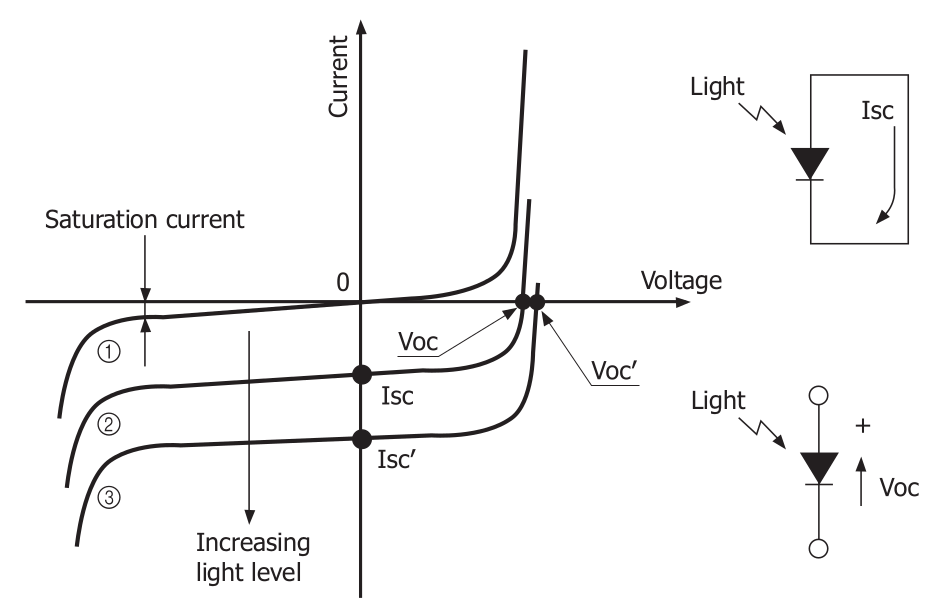
\includegraphics[width=11cm]{pdo.png}
 \end{center}
 }
 {%answer
 L'impédance d'entrée de l'AO est quasi infinie, par conséquent le courant circulant dans la diode est nul. Le point de fonctionnement est donc sur la demi-droite $[(0,0); (V>0,0)]$, par exemple $v_{oc}$ ou $v_{oc}'$.
 }

\Question
{
%question
\label{Q:ampli}
Sachant que le produit gain--bande passante de l'amplificateur utilisé vaut $10^6$Hz et que la bande passante doit être supérieure à 100kHz, dimensionnez R1 et R2 pour maximiser le gain.
}
{%answer
$GBW=10^6$, $BW=10^5Hz$ donc $G_{max}=10$, amplificateur non-inverseur, $G=1+R2/R1$ donc $R2=9\cdot R1=9k\Omega$.
Étant donné qu'on ne donne pas davantage de contrainte sur les résitances, on peut choisir une valeur arbitrairement pour $R_1$ ou $R_2$ ($R_1 = 1k\Omega$ dans notre cas).
}

 \subsubsection{Flux lumineux reçu}
 On souhaite pouvoir différentier le clignotement de la LED par rapport à l'éclairage ambiant.

% Considérons dans un premier temps un éclairage standard comme suit :
 \begin{center}
 %\shorthandoff{:!}
 		\begin{circuitikz}%\draw
 			\draw		
 			(0,0) to [sinusoidal voltage source, l=$E$] (0,2)--(2,2) to [lamp, l=$R$] (2,0) --(0,0)
 %			(1,1) to [battery1,l=$E$](1,6)
 			;
 		\end{circuitikz}
 		%\shorthandon{:!}
 	\end{center}

 \Question
 {
 %question
 En considérant la lampe comme une charge purement résistive, démontrez que la puissance consommée (et par conséquent le flux lumineux émis) contient une composante continue et une composante alternative à 100Hz. Un raisonnement utilisant un graphique peut vous aider.\\
 $E=311 \cdot sin(2\cdot\pi\cdot50t) V, R=311\Omega$

 }
 {%answer
 On peut résoudre en temporel :% ou en phaseurs
 
 $p(t)=E(t)^2/R=311\cdot\sin^2(2\pi\cdot50t) W=\frac{311}{2}\cdot(1-cos(2\pi\cdot100t))$.

En phaseurs :
 $P=E^2/R=E^2\cdot e^{2j\omega}/R$, qui a une moyenne temporelle $>0$

 Ce qui permet de conclure que le flux lumineux émis par la lampe comporte une composante continue et une composante alternative à 100Hz.
 }
%\vspace*{-0.5cm}
\enlargethispage{0.5cm}
 \Question
 {
 %question
 Qu'en est-il pour l'éclairage naturel (soleil) ?

 }
 {%answer
 L'éclairage solaire est constant au premier ordre (même si la couverture nuageuse fait apparaître des fréquences $<<1Hz$ dans le spectre).
 }
 
\subsection{Filtre}
On fixe le seuil de détection à 0.1\%, c'est à dire que la variation due au clignotement de la LED mesurée au niveau de la photodiode doit être supérieure à 0.1\% de l'éclairage ambiant pour que le faisceau soit considéré comme établi. En dessous de 0.1\% (ou si un obstacle occulte le faisceau), on considère le faisceau comme interrompu.

L'éclairage ambiant est tel que la photodiode produit une tension de 0.5V. La tension produite est une combinaison entre une composante continue et une composante alternative à 100Hz due à l'alimentation alternative des lampes. Le système doit fonctionner dans le cas extrème où l'éclairage ambiant est uniquement alternatif (0.5V, 100Hz).

La lumière de la LED de l'émetteur s'ajoute à l'éclairage ambiant. On décide que le faisceau lumineux entre l'émetteur et le récepteur est établi si la composante qui correspond à la LED a une amplitude supérieure à 0.5mV (0.1\% de l'éclairage ambiant) dans la tension produite par la photodiode.

Pour simplifier la résolution, 
 les contributions à la tension produite par la photodiode sont :
 \begin{itemize}
 \item éclairage ambiant : 0.5V, continu
 \item éclairage ambiant : composante alternative 0.5V, 100Hz, sinusoïdale
 \item LED de l'émetteur : 0.5mV, 10kHz, tension en créneaux (0--0.5mV, rapport cyclique 10\%)
 \end{itemize}
\vspace*{4mm}

 \Question
 {
 %question
 Pour conserver la composante correspondant à la LED et atténuer les composantes de l'éclairage ambiant :
 \begin{itemize}
 \item quel type de filtre utiliser ?
 \item spécifiez ses caractéristiques (ordre, gain, fréquences\dots)
 \end{itemize}
 
 Aide : la fréquence la plus haute de l'éclairage ambiant doit avoir une amplitude inférieure à 0.1\% en sortie du filtre. La fréquence correspondant à la LED ne doit pas être atténuée significativement.

 }
 {%answer
 Il faut que l'atténuation à 10kHz soit $\leq 3dB$ et l'atténuation à 100Hz $>60dB$ (=0.1\%). Il y a 2 décades entre les deux fréquences, pour respecter les contraintes, il faut un filtre d'ordre 2, passe-haut. Sa fréquence de coupure doit être $\leq 10kHz$ telle que les 60dB d'atténuation soient respectés.

 }


\Question
{
%question
Soit le filtre suivant :

\vspace*{-1cm}
\begin{center}
%\shorthandoff{:!}
		\begin{circuitikz}[scale=0.8]%\draw
			\draw		
			(0,0) to [open, v^>=$v_{in}$,o-o] (0,4) to [C,l=$22nF$] (2,4) to [L,l=$12mH$]  (2,2) to [R,l=$82\Omega$](2,0) to [short](0,0)
			(2,4) -- (4,4) to [open, v^<=$v_{out}$,o-o] (4,0) -- (2,0)
			;
		\end{circuitikz}
		%\shorthandon{:!}
	\end{center}

Déterminez le module de la fonction de transfert à 100Hz et à 10kHz. Que pouvez-vous conclure sur ce filtre ?
}
{%answer
$$\underline{V}_{out}=\underline{V}_{in}\dfrac{R+j2\pi f\cdot L}{R+j2\pi f\cdot L+1/\left(j2\pi f\cdot C\right)}$$
à 100Hz :
$\left| \dfrac{\underline{V}_{out}}{\underline{V}_{in}} \right| = 1.13e-3=-58.8dB$

à 10kHz :
$\left| \dfrac{\underline{V}_{out}}{\underline{V}_{in}} \right| = 8.66=18.75dB$

C'est un filtre passe-haut passif du deuxième ordre. Ce circuit RLC présente un phénomène de résonnance (le gain du filtre passif dépasse 1 à 10kHz)

La contrainte sur le filtre de la question précédente est respectée.
}
\enlargethispage{0.5cm}
\newpage
 \subsubsection{Gain de la chaîne}

 Les 0.1\% (0.5mV@10kHz) que représentent le clignotement de la LED au niveau de la photodiode doivent être amplifiés pour obtenir une amplitude de 6V à l'entrée du comparateur.

 \Question
 {
 %question
 En tenant compte du gain de 10 du premier étage, du gain de 8.66 apporté par le filtre RLC à 10kHz, déterminez le gain nécessaire pour respecter le cahier des charges (BW de cet étage=10kHz). En utilisant un amplificateur du même modèle que celui utilisé à la question \ref{Q:ampli}, combien d'étages supplémentaires sont nécessaires ?

 }
 {%answer
 Gain total : 12000

 Gain du premier étage +filtre à 10kHz : 86.6

 Gain nécessaire : 12000/86.6=138.6

 Le gain maximum par étage est de 100 (puisque le GBP est de $10^6$), par conséquent deux étages supplémentaires sont suffisants.
 }

\subsection{Comparateur}
Un fois le signal amplifié et filtré, il faut vérifier si son amplitude est suffisante. Un comparateur de tension est suffisant pour cette tâche.
\Question
{
Tracez le schéma d'un circuit permettant de comparer une tension avec une tension continue de 5 V.
}
{%answer
Pour réaliser un comparateur, on peut utiliser un ampli-op en saturation.

\begin{center}
	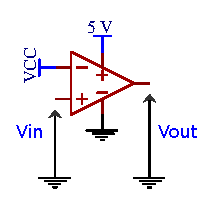
\includegraphics[scale=1.4]{comparateur.pdf}
\end{center}

En connectant le signal de référence sur l'entrée inverseuse et le signal à comparer sur l'entrée non-inverseuse, on peut exploiter la gain différentiel de l'ampli-op $A_d \cdot (V_+ - V_-)$ afin que la sortie vaille 0~V lorsque $V_{in} < VCC$ et 5~V lorsque $V_{in} > VCC$.
}
%
\subsection{Logique}
Le faisceau lumineux étant modulé, il est nécessaire d'éffectuer une démodulation du signal reçu. 

Lorsque le signal a été comparé avec le seuil, le signal obtenu est identique au signal fourni par la source de l'émetteur (si le faisceau est établi, sinon nul), un circuit logique est nécessaire pour transformer ce signal en créneaux en un signal logique représentant l'information "Pas d'obstacle". Ce circuit peut accèder à la source de l'emetteur.

On dispose de deux signaux :

\begin{itemize}
\item la source alimentant la LED de l'émetteur: signal en créneau 0--5V, 10kHz, rapport cyclique 10\%
\item la sortie du comparateur, qui est le \textbf{même} signal en créneaux (si le faisceau émetteur-récepteur est établi), 0V sinon
\end{itemize}

\Question
{
Tracez le schéma d'un circuit permettant d'obtenir le comportement suivant :

\begin{itemize}
\item La sortie passe à 1 lorsque la sortie du comparateur vaut 1
\item La sortie passe à 0 lorsque la source alimentant la LED vaut 1(=5V), sauf si la sortie du comparateur vaut 1 au même moment.
\item La sortie conserve sa valeur précédente dans les autres cas
\end{itemize}

}
{%answer
Circuit RS à Set prioritaire :
\begin{itemize}
\item S = sortie du comparateur
\item R = source alimentant la LED
\end{itemize}
}


 \Question
 {
 On désire également avoir une sortie qui marque l'éblouissement du capteur, c'est-à-dire quand la sortie du comparateur vaut 1 quel que soit l'état de la source alimentant la LED. Les contraintes sont :
 \begin{itemize}
 \item La sortie passe à 1 si la sortie du comparateur vaut 1 \textbf{et} que la source alimentant la LED vaut 0.
 \item La sortie passe à 0 si la source alimentant la LED vaut 0 sauf si la condition précédente est vraie.
 \end{itemize}

 }
 {%answer
 Circuit RS à Set prioritaire :
 \begin{itemize}
 \item  S = sortie du comparateur AND NOT  (source alimentant la LED)
 \item  R = NOT(source alimentant la LED)
 \end{itemize}
 }

\end{document}
